%% LyX 2.2.4 created this file.  For more info, see http://www.lyx.org/.
%% Do not edit unless you really know what you are doing.
\documentclass[english]{article}
\usepackage{lmodern}
\usepackage[T1]{fontenc}
\usepackage[latin9]{inputenc}
\usepackage{geometry}
\usepackage{amsmath}
\geometry{verbose,tmargin=3cm,bmargin=3cm,lmargin=2.5cm,rmargin=2.5cm}
\usepackage{textcomp}
\usepackage{float}
\usepackage{graphicx}
\graphicspath{{figures_ftr/}}

\makeatletter

%%%%%%%%%%%%%%%%%%%%%%%%%%%%%% LyX specific LaTeX commands.
%% Because html converters don't know tabularnewline
\providecommand{\tabularnewline}{\\}

\makeatother

\usepackage{babel}
\begin{document}

\title{3F8: Inference\\
 Full Technical Report}

\author{Shanzi (Monica) Ran}
\maketitle
\begin{abstract}

In this report, full Bayesian binary classification is implemented and tested via Laplace approximation. The predicitive capability of the model is examined alongside comparative metrics of average log-likelihood and confusion matrix, and a comparison with the MAP solution demonstrates the improvement in performance of the probabilistic approach.
Tuning of hyperparameters is also experimented using grid search method, which produces more flexible decision contours while being stronger against overfitting.

\end{abstract}

\section{Introduction} \label{sec:intro}
Binary classification is a fundamental problem in machine learning, where decision boundaries are developed to correctly predict the label of a new data point.Binary classification stands as a cornerstone challenge in machine learning: establishing decision boundaries that accurately predict binary outcomes for new observations. While logistic regression serves as an effective baseline for linearly separable data, its limitations become apparent when confronted with complex, non-linear patterns. Previous exercises have demonstrated that probabilistic approaches offer superior flexibility in generating decision contours for these intricate datasets.

This report examines full Bayesian regression with Laplace approximation as an alternative to traditional logistic and MAP models. Through comparative analysis of predictive performance and evaluation metrics, it is investigated how this probabilistic framework handles uncertainty. Furthermore, hyperparameter optimization via grid search is also explored to enhance model characteristics and decision boundary adaptability across varying data complexities.
\section{Exercise a)} \label{sec:exercise_a}
The normalisation of posterior probabilities is straightforward for conjugate Gaussian pairs, where the model evidence $Z=p(y|X)=\int p(y|X, \beta)p(\beta)d\beta$ can be directly calculated.
However, non-conjugate distributions pose a significant challenge as the posterior shape is not predefined. 
Laplace approximation resolves this issue by fitting a Gaussian $q(\beta)$ at the posterior's local maximum, efficiently approximating the model evidence Z needed for Bayesian logistic regression.

\subsection{Bayesian logistic regression}
The posterior distribution of model weights $\beta$ given the data $y$ and $X$ is defined by Bayes' Theorem as:
\begin{equation*}
    p(\beta|y, X) = \frac{p(y|X, \beta)p(\beta)}{p(y|X)}
\end{equation*}
where $p(y|X, \beta)$ is the likelihood, $p(\beta)$ is the prior distribution, and $p(y|X)$ is the model evidence or marginal likelihood.
For model simplicity, the prior is assumed to be Gaussian with zero mean and variance $\sigma_0^2$, and the likelihood is chosen as Bernoulli with the logistic sigmoid function $\sigma(\beta^T\phi)$.
Denoting $\mathbf{S}_0=\sigma_0^2\mathbf{I}$, the Gaussian prior is formalised as $p(\beta)=\mathcal{N}(\beta|0, \mathbf{S}_0)$ to unify matrix shape and expressions.

\subsection{Laplace approximation of the posterior distribution $p(\beta|y, X)$}
The expression of the Laplace approximation $q(\beta)$ can be found using the truncated Taylor expansion. Around the mode $\beta_0$ where $\frac{df(\beta)}{d\beta}\Big|_{\beta=\beta_0}=0$, monoticity of the logarithm function gives $\nabla \log f(\beta)=0$, hence:
\begin{equation*}
    \log f(\beta) \simeq \log f(\beta_0) - \frac{1}{2} \mathbf{A} (\beta - \beta_0)^2, \quad \mathbf{A}=-\nabla^2\log f(\beta)\big|_{\beta=\beta_0}
\end{equation*}

Restoring to exponential form yields a Gaussian distribution centered at $\beta_0$, which is identified using Maximum A Posteriori (MAP) estimation. With $\beta_0 = \beta_{MAP}$, the covariance of this Gaussian is defined by the Hessian matrix $\mathbf{S}_N^{-1}=-\nabla^2 \log f(\mathbf{\beta})\big|_{\mathbf{\beta}=\mathbf{\beta}_{MAP}}$. Standard Gaussian normalization method is then applied to yield the posterior approximation:
\begin{equation} \label{posterior_approximation}
    p(\beta|y, X) \approx q(\beta) = \mathcal{N}(\mathbf{\beta}|\mathbf{\beta}_0, \mathbf{S}_N^{-1}) = \frac{1}{(2\pi)^{\frac{N}{2}} \det \mathbf{S}_N^{-\frac{1}{2}}} \exp\{\frac{1}{2} (\beta - \beta_{MAP})^T \mathbf{S}_N^{-1}(\beta - \beta_{MAP})\}.
\end{equation}
Using this expression, the Hessian matrix can be simplified as:
\begin{equation}
    \mathbf{S}_N^{-1} = -\nabla^2 \log p(\beta|y, X) = \mathbf{S}_0 + \sum_{n=1}^{N} \sigma(\beta^Tx_n)(1-\sigma(\beta^T x_n))x_n x_n^T
\end{equation}

\subsection{Approximated log model evidence}
Using the approximated posterior distribution, the log model evidence can then be calculated as:
\begin{align} 
    \log p(y|X) &= \log \int p(y|X, \beta)p(\beta)d\beta \notag \\
    &\approx \log p(y|X, \beta_{MAP}) + \log p(\beta_{MAP}) - \frac{1}{2} \log |\mathbf{S}_N^{-1}| + \frac{N}{2} \log 2\pi \label{log_model_evidence}
\end{align}
which is a combination of the log prior, log likelihood, and the negative log of the determinant of the inverse covariance matrix for the posterior.

\subsection{Approximated predictive distribution}
For the binary classification problem concerned in this exercise, the predictive distribution is then obtained by marginilising the approximated posterior probability obtained in Equation~\ref{posterior_approximation}. For category $\mathcal{C}_1$, given a new feature vector $\phi(x)$:
\begin{equation} \label{predictive_distribution}
    p(\mathcal{C}_1|\phi, y, X) = \int p(\mathcal{C}_1|\phi, \beta)p(\beta|y, X)d\beta 
    \simeq \int \sigma(\beta^T \phi)q(\beta)d\beta 
\end{equation}

Simplifying Equation~\ref{predictive_distribution} using the sifting property of Dirac delta function:
\begin{equation*}
    p(\mathcal{C}_1|\phi, y, X) = \int \sigma(\beta^T\phi)\mathcal{N}(\beta^T\phi|\beta_{MAP}^T\phi, \phi^T \mathbf{S}_N\phi) = \int \sigma(\beta ^T \phi)\mathcal{N}(\mu_{pred},\sigma_{pred}^2)d\beta
\end{equation*}

so $\mu_{pred}=\beta_{MAP} ^T \phi$, $\sigma_{pred}^2=\phi^T \mathbf{S}_N \phi$. This can be further simplified by approximating the logistic sigmoid with prodit function $\Phi(\lambda x)$ with the scale factor $\lambda ^2 = \pi / 8$:
\begin{equation}
    p(\mathcal{C}_1|\phi, y, X) = \sigma(\kappa(\phi^T S_N\phi)\beta^T\phi|\beta_{MAP}^T\phi), \quad \kappa(\sigma ^2) = (1+\pi \sigma^2 / 8)^{-1/2}
\end{equation}

\section{Exercise b)}
Given the posterior distribution in Equation~\ref{posterior_approximation}, the gradient of the log-posterior can be calculated as a combination of the gradient of the log-prior and log-likelihood:
\begin{equation}\label{log_posterior_gradient}
    \nabla \log p(\beta|y, X) =  \nabla \log p(\beta) + \sum_{n=1}^{N} \{y_n - \sigma(\beta^T x_n)\}x_n
    = \sum_{n=1}^{N} \{y_n - \sigma(\beta^T x_n)\}x_n - \mathbf{S}_0^{-1}\beta
\end{equation}
which can be used to obtain the MAP solution $\beta_{MAP}$ by setting the gradient to zero. In this exercise, this optimisation is performed using \texttt{scipy.optimize.fmin\_l\_bfgs\_b} method, which is a limited-memory quasi-Newton optimisation algorithm that effectively minimises the negative log-posterior gradient subject to simple box constraints.

Summarising equations demonstrated in Section~\ref{sec:exercise_a}, the Python code implementation of the Laplace approximation is provided below:

\begin{itemize}
    \item \texttt{neg\_log\_posterior}: Function that calculates the negative log-posterior given the model weights, data, and prior hyperparameters.
    \begin{verbatim}
    def neg_log_posterior(w, X_tilde, y, S, m0):
        k = predict(X_tilde, w)
        log_prior = -0.5 * np.dot(np.dot(w-m0, np.linalg.inv(S)), w-m0)
        ll = np.sum(y * np.log(k) + (1 - y) * np.log(1-k))
    
        return -(ll + log_prior)
    \end{verbatim}

    \item \texttt{grad\_neg\_log\_posterior}: Function that calculates the gradient negative log-posterior given the model weights, data, and prior hyperparameters, according to Equation~\ref{log_posterior_gradient}. The output is used for the \texttt{fmin\_l\_bfgs\_b} method.
    \begin{verbatim}
    def grad_neg_log_posterior(w, X_tilde, y, S, m0):
        k = predict(X_tilde, w)
        log_prior_grad = - np.dot(np.linalg.inv(S), w) + np.dot(np.linalg.inv(S), m_0)
        ll_grad = X_tilde.T @ (y - k)
        
        return -(log_prior_grad + ll_grad)
    \end{verbatim}

    \item \texttt{grad\_neg\_log\_posterior}: Function that computes the Hessian matrix (not inverse) of likelihood given the model weights and data. This is used for defining the approximated Gaussian posterior.
    \begin{verbatim}
    def hessian_ll(w, X_tilde, y):
        k = predict(X_tilde, w)
        h_ll = np.zeros((len(w), len(w)))
        
        for i, x in enumerate(X_tilde):
            ki = k[i]
            h_ll += np.outer(x, x) * ki * (1 - ki)
        
        return h_ll
    \end{verbatim}

    \item \texttt{grad\_neg\_log\_posterior}: Function that performs the Laplace approximation using the above defined functions and \texttt{fmin\_l\_bfgs\_b} method. The output is the MAP solution of the model weights, the covariance matrix of the Laplace approximation, and the log model evidence.
    \begin{verbatim}
    def laplace_approx(X_tilde, y, S, m0):
        D = X_tilde.shape[1]
        w0 = np.zeros(X_tilde_train.shape[1])
        w_map, fmin, _ = fmin_l_bfgs_b(neg_log_posterior, w0, fprime=grad_neg_log_posterior, args=(X_tilde, y, S, m0))
    
        H = np.linalg.inv(S) + hessian_ll(w_map, X_tilde, y)
        S_N = np.linalg.inv(H) # Covariance matrix of Laplace approximation
    
        # Compute model evidence using approximation
        H += 1e-6 * np.eye(H.shape[0]) # For numerical stability
        sign, log_det_H = np.linalg.slogdet(H)
        if sign <= 0:
            return w_map, S_N, -np.inf  # Reject when Hessian is not positive semi-definite
        log_posterior = -neg_log_posterior(w_map, X_tilde, y, S, m0)
        log_evidence = log_posterior - 0.5 * log_det_H
    
        return w_map, S_N, log_evidence
    \end{verbatim}

    \item \texttt{kappa}: Helper function that approximates the logistic sigmoid function using the probit function.
    \begin{verbatim}
    def kappa(var): return (1 + np.pi * var / 8)**0.5
    \end{verbatim}

    \item \texttt{laplace\_prediction}: Function that computes the predictive distribution using the Laplace approximation. The output is the class predictive probabilities.
    \begin{verbatim}
    def laplace_prediction(X_tilde, w_map, S_N):
        pred_mean = X_tilde @ w_map
        pred_var = np.array([x @ S_N @ x for x in X_tilde])
        return logistic(pred_mean / kappa(pred_var))
    \end{verbatim}

    \item \texttt{bayesian\_prediction}: Function that computes the predictive distribution directly using the MAP solution, which serves as a control for the Laplace approximation. This function is adjusted from \texttt{predict} in order to line-up with the implementation.
    \begin{verbatim}
    def bayesian_prediction(X_tilde, w_map, S_N): return logistic(np.dot(X_tilde, w_map))
    \end{verbatim}
\end{itemize}

\section{Exercise c)}
The predictive contours generated by the Laplace approximation and the MAP solution are shown in Fig~\ref{fig:predictive_distributions}.
Both predictions are generated using the same prior distribution of $\mathcal{N}(0, 1)$ and the RBF width $l=0.1$, and only differ by the prediction algorithm. 
As can be observed from the contour maps, the Laplace full Bayesian approximation provides very similar results to the MAP solution, and differences are hardly visually distinguishable.
In some areas the Laplace approximation provides a slightly more conservative predictions where neighbouring contour lines are more spread out, indicating a higher uncertainty in the prediction.
This observation aligns with the theoretical understanding of the Laplace approximation, where the installation of the prior Gaussian distribution helps avoid overfitting by accounting for parameter variabilities.
It is also worth noting that this difference would be enlarged if the prior variance is increased.

\begin{figure}[H]
\begin{centering}
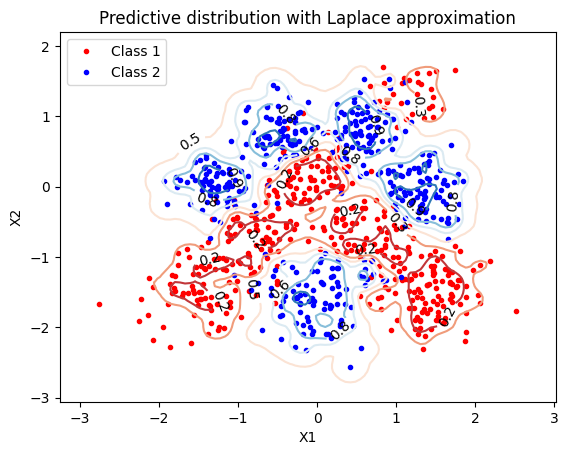
\includegraphics[width=0.3\paperwidth]{c_laplace.png}\hspace{1cm}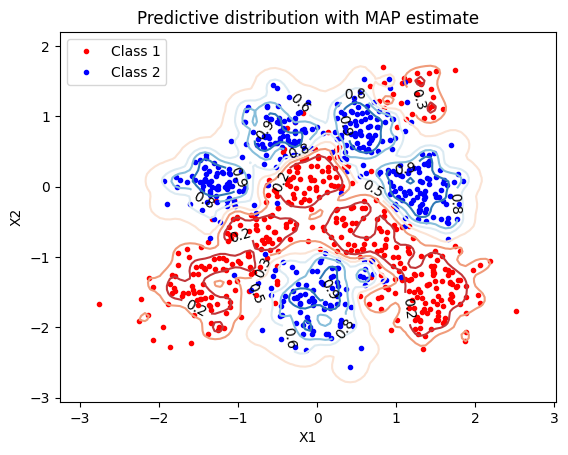
\includegraphics[width=0.3\paperwidth]{c_map.png}
\par\end{centering}
\caption{Plots showing data and contour lines for the predictive distribution
generated by the Laplace approximation (left) and the MAP solution
(right).\label{fig:predictive_distributions} }
\end{figure}


\section{Exercise d)}
Table~\ref{tab:ll_MAP} and Table~\ref{tab:ll_Laplace} show the average training and test log-likelihoods for the MAP solution and the Laplace approximation.
It can be observed that the full Bayesian method via Laplace approximation provide slightly smaller log-likelihoods for both the training and test datasets comparing to those obtained for the MAP solution.
This could also help explain the more conservative prediction contours in Fig~\ref{fig:predictive_distributions} as the prior prevents overfitting to the data. 
For both methods, the final average log-likelihoods on the training dataset converges to a higher value than that of the test dataset, aligning with observations made from simple logistic classifiers in the previous exercise.

\begin{table}[H]
\centering{}%
\begin{minipage}[t]{0.5\textwidth}%
\begin{center}
\begin{tabular}{c|c}
\textbf{Avg. Train ll} & \textbf{Avg. Test ll}\tabularnewline
\hline 
$-0.220$ & $-0.293$\tabularnewline
\hline 
\end{tabular}\caption{Log-likelihoods for MAP solution.\label{tab:ll_MAP}}
\par\end{center}%
\end{minipage}%
\begin{minipage}[t]{0.5\textwidth}%
\begin{center}
\begin{tabular}{c|c}
\textbf{Avg. Train ll} & \textbf{Avg. Test ll}\tabularnewline
\hline 
$-0.260$ & $-0.318$\tabularnewline
\hline 
\end{tabular}\caption{Log-likelihoods for Laplace approximation.\label{tab:ll_Laplace}}
\par\end{center}%
\end{minipage}
\end{table}

Another important evaluation metric for regression classifiers is the confusion matrix, as the results are shown below in Table~\ref{tab:conf_MAP} and Table~\ref{tab:conf_Laplace}.
It is noticeable that the confusion matrices are identical for both the MAP solution and the Laplace approximation, indicating identical decision boundaries.
This is expected as both methods are based on the same $\beta_{MAP}$ mean. The differences in predictive contours originate from the covariance matrix $\mathbf{S}_N$ in the Laplace approximation that defines how the full Bayesian approach develops a probability distribution of weights around this mean, which is not reflected in the confusion matrix.
\begin{table}[H]
\centering{}%
\begin{minipage}[t]{0.5\textwidth}%
\begin{center}
\begin{tabular}{cc|c|c}
 & \multicolumn{1}{c}{} & \multicolumn{1}{c}{$\hat{y}$} & \tabularnewline
 &  & 0 & 1\tabularnewline
\cline{2-4} 
$y$ & 0 & $0.949$ & $0.051$\tabularnewline
\cline{2-4} 
 & 1 & $0.059$ & $0.941$\tabularnewline
\cline{2-4} 
\end{tabular} 
\par\end{center}
\caption{Conf. matrix for for MAP solution.\label{tab:conf_MAP}}
%
\end{minipage}%
\begin{minipage}[t]{0.5\textwidth}%
\begin{center}
\begin{tabular}{cc|c|c}
 & \multicolumn{1}{c}{} & \multicolumn{1}{c}{$\hat{y}$} & \tabularnewline
 &  & 0 & 1\tabularnewline
\cline{2-4} 
$y$ & 0 & $0.949$ & $0.051$\tabularnewline
\cline{2-4} 
 & 1 & $0.059$ & $0.941$\tabularnewline
\cline{2-4} 
\end{tabular} 
\par\end{center}
\caption{Conf. matrix for Laplace approximation.\label{tab:conf_Laplace}}
%
\end{minipage}
\end{table}


\section{Exercise e)}
As seen in Equation~\ref{log_model_evidence}, the model evidence estimate using the Laplace approximation increases with log-likelihood and log-prior, while decreasing with the determinant of $\textbf{S}_N^{-1}$ matrix. The constant term $\frac{N}{2} \log 2\pi$ is ignored in the optimisation process as it does not affect the comparison between different models.
This equation for the log-evidence relating the two hyperparameters also specifies the tradeoff between the fit to the data, represented by log-likelihood, and the complexity of the model, which is expressed by the determinant of Hessian matrix.
Thus, the model can be optimised without overfitting by maximising the model evidence, where the complexity term is penalised.

In this exercise, this optimisation is performed together with tuning of the RBF width $l$ using a simple grid search method. 
The Python code implementation is provided below:
\begin{verbatim}
def hp_tune(X_train, y_train, m_0, sigmas, ls):
    l_opt = 0
    sigma_opt = 0
    log_evidence_opt = -np.inf

    log_evidence_list = np.zeros((len(sigmas), len(ls)))

    for i, l in enumerate(ls):
        X_tilde_train = get_x_tilde(evaluate_basis_functions(l, X_train, X_train))
        for j, sigma in enumerate(sigmas):
            S = (sigma ** 2) * np.eye(X_tilde_train.shape[1])
            print(f"l: {l}, sigma: {sigma}")
            log_evidence = laplace_approx(X_tilde_train, y_train, S, m_0)[2]
            log_evidence_list[i][j] = log_evidence

            if log_evidence > log_evidence_opt:
                l_opt = l
                sigma_opt = sigma
                log_evidence_opt = log_evidence
            
            print(f"Evidence: {log_evidence_list[i][j]}")
            
    return l, sigma, log_evidence_opt, log_evidence_list, ls, sigmas
\end{verbatim}

The grid search process above defined is conducted in two runs, where a coarse-scale search is first performed to locate the approximate range of optimal values, followed by a second search with higher precision. Both searches are maintained at a \texttt{10 * 10} grid for computational simplicity.
As linear grid points fail to establish useful information in trail runs, a logarithmic scale is adopted and shown in Fig~\ref{fig:grid_search}. The fine-scale ranges located are $ 10^{-0.01} < \sigma_0 < 10^{0.02} $ and $ 10^{-0.35} < l < 10^{-0.2} $. 
According to graphical visualisations, the optimum is chosen to be $\sigma_0^2 = (10^{0.02})^2 = 1.096 $ and $l = 0.446 $ for balance of stability and performance with reference to the hyperparameters tested in experiments recorded above.

One noticeable observation from the grid search result is that optimisation of the log evidence with respect to the prior variance is not as efficient as expected, especially when comparing to the clearer trends established for the RBF width.
It is observed that as the prior variance increases, the log-evidence always improves for both the wide and narrow range.
This is suspected to be caused by the reward of overfitting exceeding the penalty as $\sigma_0^2$ increase. As the prior approaches a more uniform distribution, the expected constraining effect on the likelihood growth diminishes.

While the grid search method did not yield reliable optimisation results, another approach optimising with respect to the prior precision by calculating the trace of the $\textbf{S}\_N^{-1}$ is also tested. Expressing the derivative of the log-determinant term as its trace $\frac{d}{d \sigma^{-1}} = \text{Trace}(\textbf{S}_N^{-1})$, the log-evidence is optimised at:
\begin{equation*}
    \sigma_{OPT} = \frac{\beta_{MAP}^T \beta_{MAP}}{\omega}, \omega = \text{Effective Degree-of-Freedom}(\textbf{S}_N)
\end{equation*}

implemented in Python as:
\begin{verbatim}
def opt_prior_variance(w_map, X_tilde, y, S_N):
    h_ll = hessian_ll(w_map, X_tilde_train, y_train)
    sigma_opt = np.dot(w_map, w_map) / np.trace(S_N * h_ll)
    return sigma_opt
\end{verbatim}
which yields an optimum prior variance $\sigma_0^2 = 0.346$, which is far from the grid search result, further illustrating that a simple grid search might not be sufficient for fully and efficiently tuning the hyperparameters.

\begin{figure}[H]
    \begin{centering}
    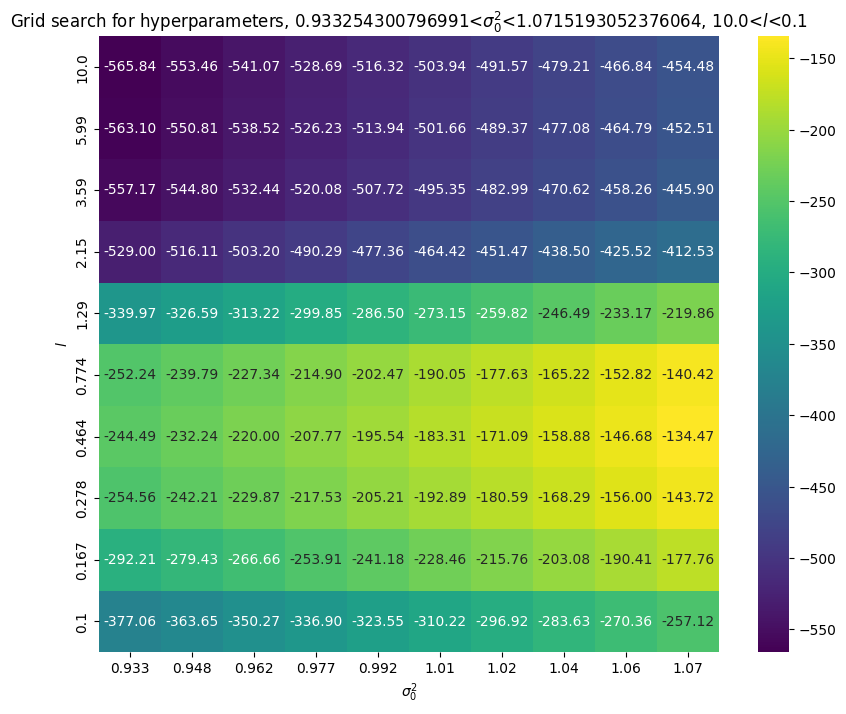
\includegraphics[width=0.3\paperwidth]{wide.png}\hspace{1cm}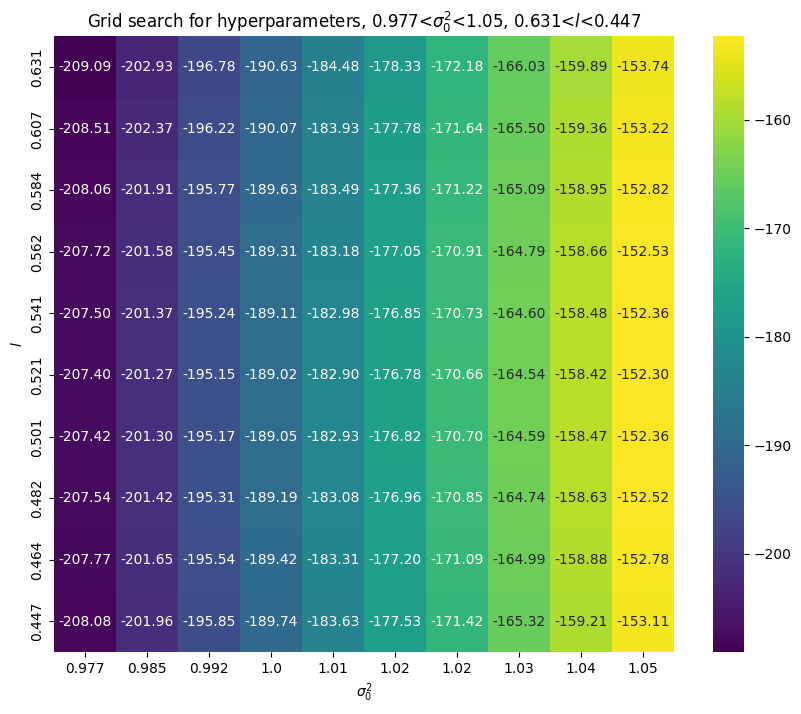
\includegraphics[width=0.3\paperwidth]{narrow.png}
    \par\end{centering}
    \caption{Plots showing data and contour lines for the predictive distribution
    generated by the Laplace approximation (left) and the MAP solution
    (right).\label{fig:grid_search} }
\end{figure}


\section{Exercise f)}
Using the optimisation results obtained in the previous section, a set of new predictive contours is displayed in Fig~\ref{fig:predictive_visualisation_after_tuning}, alongside average training and test log-likelihood data and the confusion matrix in Table~\ref{tab:average_ll_after_tuning} and Table~\ref{tab:confusion_after_tuning} respectively.
The decision contours are evidently more smooth than both the visualisations shown in Fig~\ref{fig:predictive_distributions}, which indicates less overfitting due to the tuning of hyperparameters, notably the wider RBF radius. It can also be observed that the distance between neighbouring contours lines vary further in different parts of the state space, which is captured by the increased prior variance generated by the grid search optimisation.

It can also be concluded that the average log-likelihood values increase due to the tuning for both the trainig and test datasets, where the difference between the two is also shrinking. This indicates that although the model fits the datasets better, it is not suffering from overfitting to the training data as would happen for simple logistic regressors.
Meanwhile, the confusion matrix results does not exhibit too striking differences from the before-tuning results, which might be the consequence of too small changes from the original hyperparameter settings.
\begin{figure}[H]
    \begin{centering}
    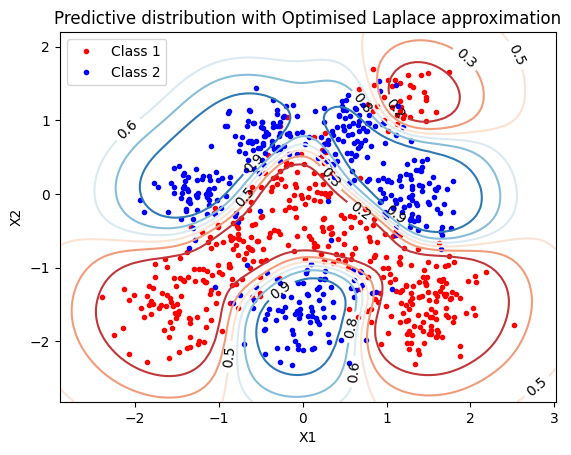
\includegraphics[width=0.5\paperwidth]{final_pred.png}
    \par\end{centering}
    \caption{Plot showing data and contour lines for the predictive distribution
    generated by the Laplace approximation with optimised hyperparameters. \label{fig:predictive_visualisation_after_tuning} }
\end{figure}

\begin{table}[H]
\centering{}%
\begin{minipage}[t]{0.4\columnwidth}%
\begin{center}
\vspace{-0.2cm}%
\begin{tabular}{c|c}
\textbf{Avg. Train ll} & \textbf{Avg. Test ll}\tabularnewline
\hline 
$-0.164$ & $-0.197$\tabularnewline
\hline 
\end{tabular} 
\par\end{center}
\caption{Average training and test log-likelihoods for Laplace approximation
after hyper-parameter tuning by maximising the model evidence.\label{tab:average_ll_after_tuning}}
%
\end{minipage}\hspace{2cm}%
\begin{minipage}[t]{0.4\columnwidth}%
\begin{center}
\begin{tabular}{cc|c|c}
 & \multicolumn{1}{c}{} & \multicolumn{1}{c}{$\hat{y}$} & \tabularnewline
 &  & 0 & 1\tabularnewline
\cline{2-4} 
$y$ & 0 & $0.934$ & $0.066$\tabularnewline
\cline{2-4} 
 & 1 & $0.077$ & $0.923$\tabularnewline
\cline{2-4} 
\end{tabular} 
\par\end{center}
\caption{Confusion matrix for Laplace approximation after hyper-parameter tuning
by maximising the model evidence.\label{tab:confusion_after_tuning}}
%
\end{minipage}
\end{table}


\section{Conclusions}
In this report, explorations to extend the simple logistic classifier to a full Bayesian classifier via Laplace approximation is recorded in progressive order.
The regularisation effect provided by the addition of the prior distribution is discussed and assessed in detail refering to both model predictive performances and computational metrics.
The full Bayesian approach outperforms the logistic regressor and MAP classifier in almost all metrics, demonstrating the effectiveness of incorporating prior knowledge and accounting for parameter uncertainty and preventing overfitting issues, providing a balance between data fitness and model complexity. 
While tuning of hyperparameters including the prior variance and RBF width is also experimented, future work is expected to perform more sophisticated strategies of more reliable and efficient optimisation of the log-evidence.
\end{document}
